\section{Aggregate-Only Reproducibility Framework}

We propose a five-layer framework for sensitive speech AI evaluation.

\begin{figure}[htbp]
\centering
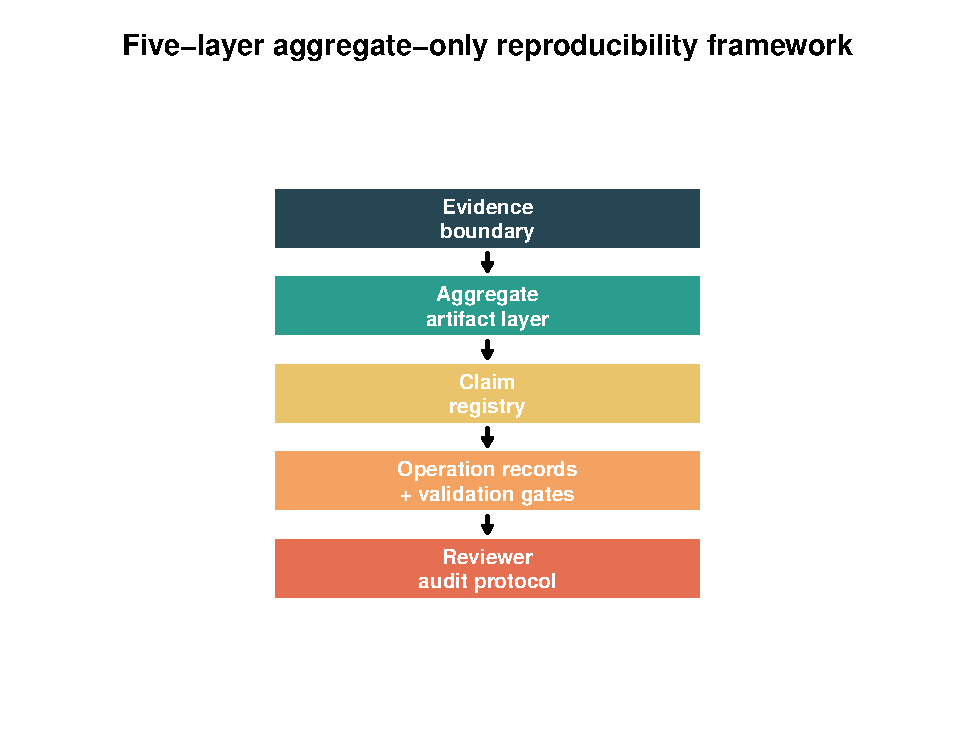
\includegraphics[width=.9\linewidth]{figures/fig1_framework_layers.pdf}
\caption{Five-layer aggregate-only reproducibility framework. The figure is generated by \artifact{paper_4b_aggregate_reproducibility/r/build_fig1_framework_layers.R} as a conceptual framework derived from the manuscript protocol.}
\label{fig:framework}
\end{figure}

\subsection{Layer 1: Evidence Boundary}

The evidence boundary defines which materials are public aggregate artifacts and which remain local-only sensitive evidence. Figure~\ref{fig:boundary} maps the boundary.

\begin{figure}[htbp]
\centering
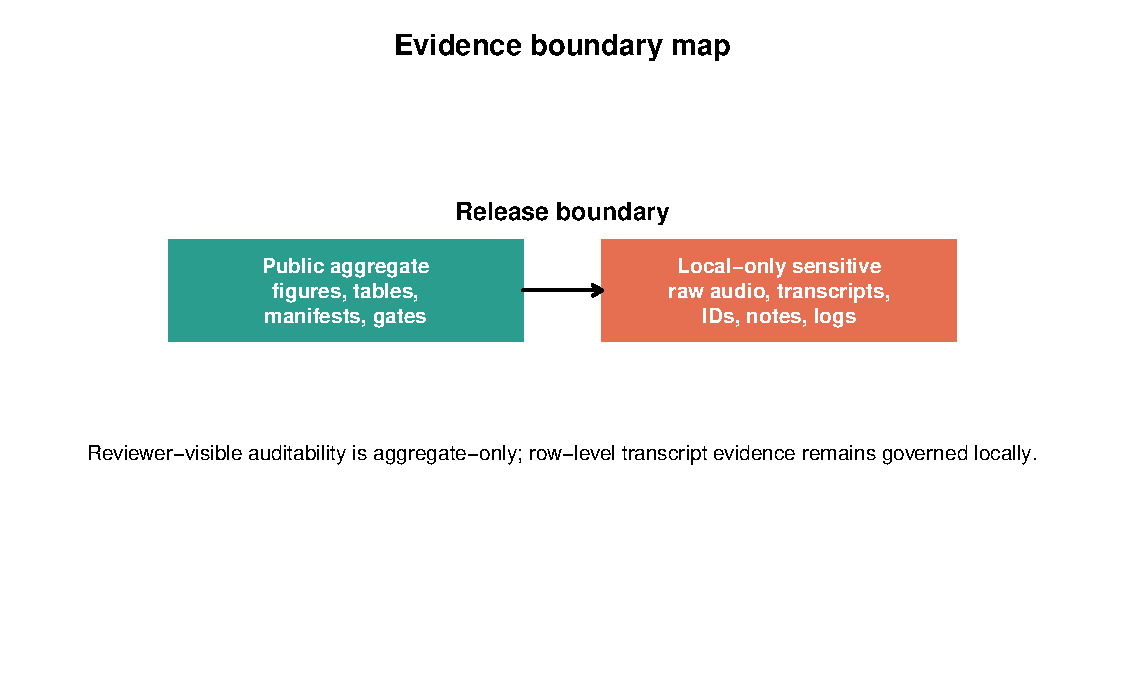
\includegraphics[width=.9\linewidth]{figures/fig2_evidence_boundary.pdf}
\caption{Evidence boundary map separating public aggregate artifacts from local-only sensitive evidence. Generated by \artifact{build_fig2_evidence_boundary.R}.}
\label{fig:boundary}
\end{figure}

\subsection{Layer 2: Aggregate Artifact Layer}

The aggregate artifact layer releases transcript-free summary tables, metric outputs, validation summaries, manifest rows, figure inputs, agreement summaries, and completion checks. Transcript-bearing rows, identifiers, reviewer notes, response sheets, model hypotheses, and transcript-bearing logs remain governed local evidence.

\subsection{Layer 3: Claim Registry}

The claim registry maps every paper-facing claim to artifact path, statistic, scope, limitation, privacy class, and validation status. Figure~\ref{fig:claim_flow} shows the claim-to-evidence flow.

\begin{figure}[htbp]
\centering
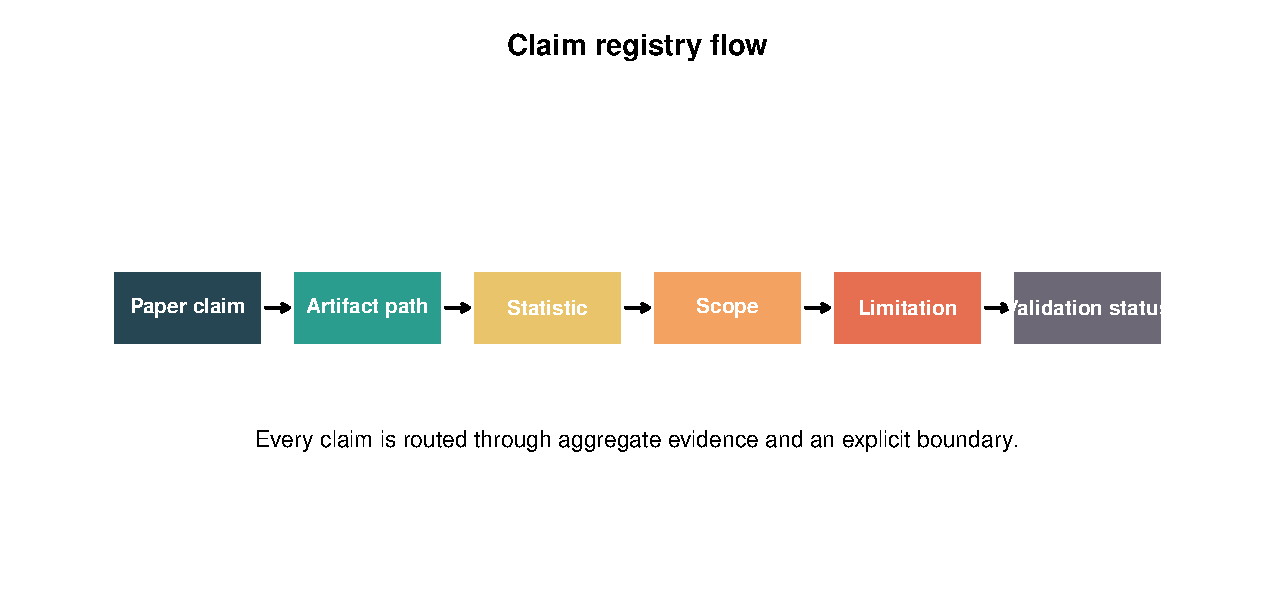
\includegraphics[width=.9\linewidth]{figures/fig3_claim_registry_flow.pdf}
\caption{Claim registry flow from paper claim to artifact, statistic, scope, limitation, privacy class, and validation status. Generated by \artifact{build_fig3_claim_registry_flow.R}.}
\label{fig:claim_flow}
\end{figure}

\subsection{Layer 4: Operation Records And Validation Gates}

Operation records and validation gates provide process-level audit trails without exposing sensitive content. They include artifact manifests, evidence-chain readiness checks, consistency checks, publishable-evidence summaries, and leak checks.

\subsection{Layer 5: Reviewer Audit Protocol}

The reviewer audit protocol specifies what reviewers can inspect: artifact completeness, claim-evidence alignment, consistency checks, metric definitions, agreement summaries, scope boundaries, and R-based figure regeneration. Row-level qualitative interpretation remains a governed local validation layer when public release would expose sensitive transcript-bearing content.
